%\counterwithin{figure}{section}

\chapter{Funzionamento dell'applicazione}

\section{Descrizione dei controller}
L’applicazione dispone di due controller:
\begin{itemize}
    \item \textbf{FXMLController}, gestisce la parte simulativa permettendo di impostare e avviare la simulazione;
    \item \textbf{RisultatiController2}, permette la visualizzazione in forma tabulare delle varie simulazioni effettuate.
\end{itemize}
\newpage
\section{Impostazione dei parametri di simulazione}
All’avvio della simulazione, verrà visualizzata la prima View \textit{Scene.fxml} (Figura \ref{fig:scene_fxml}), tramite la quale è possibile impostare i vari parametri simulativi inserendoli in caselle di testo e scegliendo tra opzioni disponibili nelle \textit{ComboBox}.

\begin{figure}[h!]
    \centering
    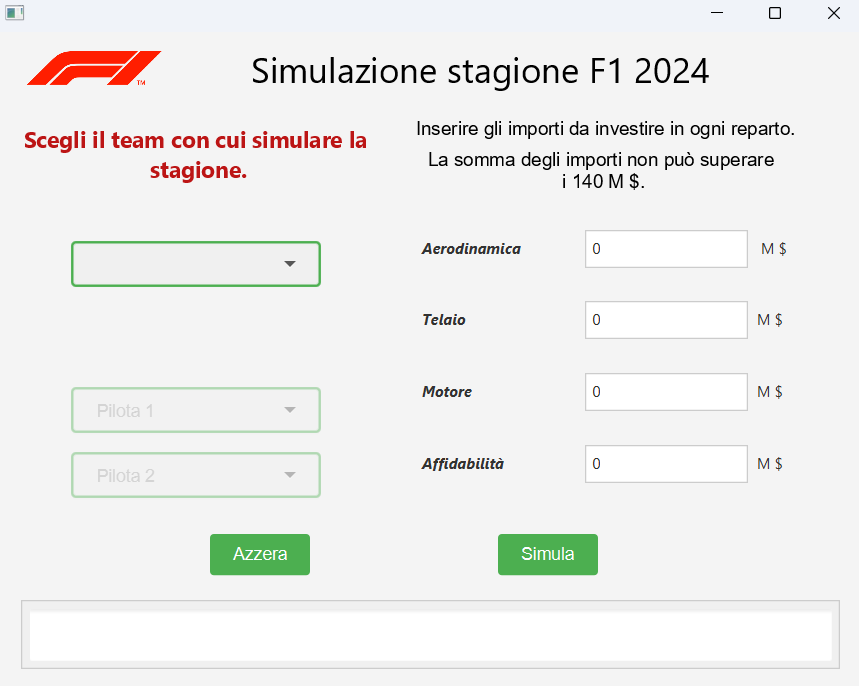
\includegraphics[width=0.8\linewidth]{Figures/schermata1.png}
    \caption{View Scene.fxml}
    \label{fig:scene_fxml}
\end{figure}

I parametri che possono essere impostati sono:
\begin{itemize}
    \item \textbf{Scuderia} in cui poter investire, tramite \textit{ComboBox};
    \item La coppia di \textbf{piloti} che gareggeranno per la scuderia scelta, tramite \textit{ComboBox};
    \item Il valore dell’\textbf{investimento} nei vari settori (\textit{Aerodinamica, Telaio, Motore, Affidabilità}), tramite caselle di testo.
\end{itemize}

L’unica limitazione riguarda la somma dei valori dell’investimento che non può superare i 140M \$. Se questa regola non è rispettata o se l’inserimento dei dati non è svolto correttamente, l’applicazione non permetterà di avviare la simulazione segnalando l’errore. Sono presenti due pulsanti, ‘\textit{Azzera}’ e ‘\textit{Simula}’, grazie ai quali è possibile ripristinare ai valori standard i vari campi editabili o iniziare la simulazione.
\newpage
\section{Visualizzazione dei risultati}
Dopo l’avvio della simulazione, si verrà trasferiti ad un’altra View \textit{Risultati2.fxml} (Figura \ref{fig:risultati_fxml}).

\begin{figure}[h!]
    \centering
    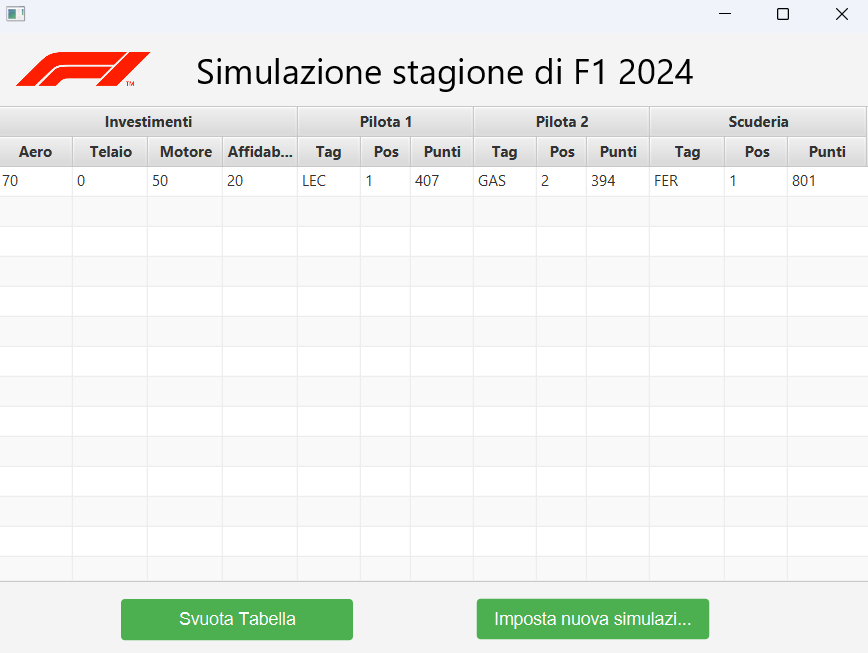
\includegraphics[width=0.8\linewidth]{Figures/singola.png}
    \caption{View Risultati.fxml}
    \label{fig:risultati_fxml}
\end{figure}

Qui sono mostrati i risultati delle varie simulazioni tramite le righe di una tabella. Tramite il pulsante ‘\textit{Avvia nuova simulazione}’ è possibile tornare alla View iniziale e impostare una nuova simulazione. Se la simulazione è stata avviata con successo, nella tabella della View \textit{Risultati.fxml} verrà aggiunta un’altra riga che riporta i dati dell’ultima simulazione. La tabella è in grado di immagazzinare e riportare i risultati di un gran numero di simulazioni, per permettere un semplice e immediato confronto.

Per ogni riga è indicata la scuderia scelta per la simulazione, i valori degli investimenti effettuati, punti e posizioni finali in classifica dei due piloti e della scuderia alla fine dell’anno. Tramite un pulsante ‘\textit{Svuota Tabella}’ è possibile cancellare tutte le righe della tabella.


